Benchmarking-delens fremmeste formål er at finde svar på en række spørgsmål
inden udregningen sættes igang. Vi præsenterer her resultaterne af en lang række prøvekørsler, hver med en kort beskrivelse af omstændigheder omkring kørslen og de udledninger vi har foretaget på baggrund af resultatet. Prøvekørslerne refereres fra de foregående afsnit, hvor det er relevant. Uddata for benchmarkkørsler er ikke inkluderet i rapporten på grund af pladshensyn. Al uddata kan hentes fra \url{http://queens.googlecode.com/svn/trunk/doc/benchmarks/}.

\subsection{Lokale tests}

Vi har 3 forskellige udgaver af koden
\begin{description}
\item[1] En direkte port, der ikke er parallelliseret.
\item[2] En parallelliseret udgave, der kører rekursivt.
\item[3] En parallelliseret udgave, der kører iterativt.
\end{description}

Disse udgaver er beskrevet mere indgående i afsnit \ref{implementering}
I dette afsnit vil der ind i mellem blive referet til noget vi har kaldt
\texttt{maxSteps}. \texttt{maxSteps} er beskrevet mere i \ref{impcornerboard} 

Vi starter med at teste de forskellige udgaver af koden lokalt, så vi har en
baseline at sammenligne med.

Alle lokale tests er kørt på en IBM T43, med en pentium m 1.86Ghz cpu, 

Java koden er kompilet med javac

\begin{verbatim}
alex@roadrunner:~/temp/queens/src/main/java$ javac -version
javac 1.5.0_11
\end{verbatim}

C koden er kompilet med \texttt{gcc -O2 -o nq nqueens.c}

\begin{verbatim}
alex@roadrunner:~/temp/queens/src/main/java$ gcc --version
gcc (GCC) 4.1.2 (Ubuntu 4.1.2-0ubuntu4)
\end{verbatim}

I de første test der brugt int til resultaterne i java-koden. 

\begin{figure}[h]
\begin{center}
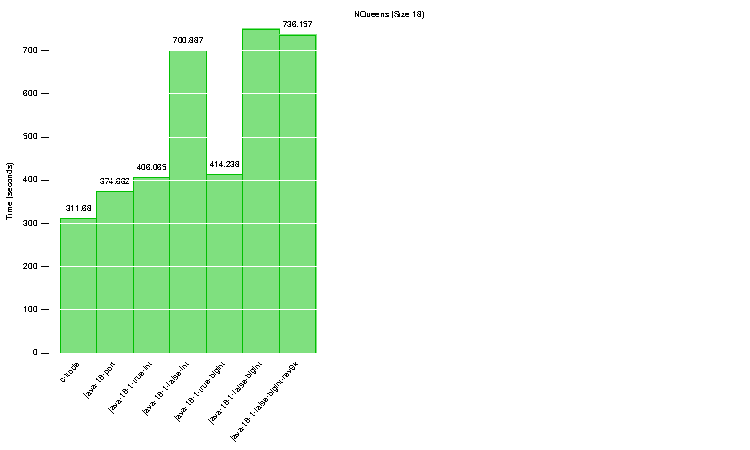
\includegraphics{../benchmarks/lokal.pdf}
\caption{Sammenligning af de lokale test} 
\label{figur:lokal}
\end{center}
\end{figure}

Som det ses er C udgaven en smule hurtigere end den direkte java port, der igen
er lidt hurtigere end den paralleliserede udgave af koden, når den kører
rekursivt. Den iterative udgave er væsentlig langsommere..

Den parallelle udgave af koden er i dette tilfælde her kørt med
\texttt{maxSteps} på 1. 

\begin{figure}[h]
\begin{center}
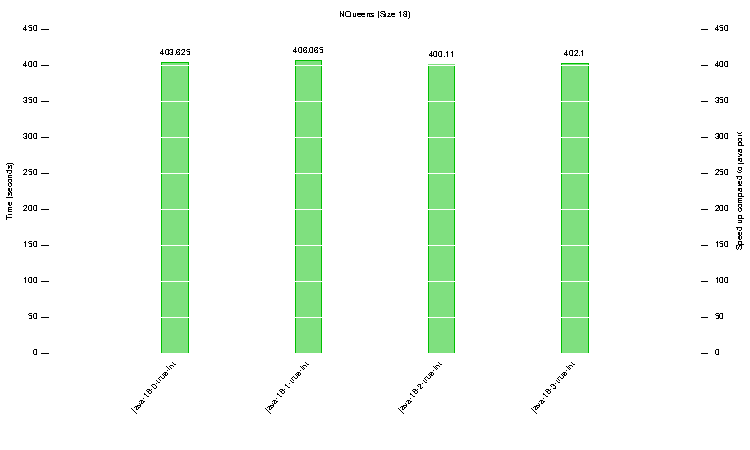
\includegraphics{../benchmarks/maxsteps.pdf}
\caption{NQueens for $n=18$ og $maxSteps=0..3$, kørt med den rekursive java-kode} 
\label{figur:maxsteps}
\end{center}
\end{figure}

På figur \ref{figur:maxsteps} er vist kørsler for $n=18$ for forskellige
$maxSteps$. 
Som det ses, har det ikke den store indflydelse på performance hvor stor
$maxSteps$ er, der er altså ikke det store overhead ved at generere en masse
opgaver og løse dem bagefter, når det kører lokalt. 




I tabel \ref{tabel:noboards} kan det ses hvor mange boards der bliver genereret
for forskellige $n$ og $maxSteps$. 

\begin{table}
	\begin{center}
		\begin{tabular}{|c|c|c|c|c|c|}
			\hline N  & maxSteps  & boards & n  & maxSteps & boards \\
			\hline 15 & 0         & 18     & 17 & 0        & 21     \\
			\hline 15 & 1         & 173    & 17 & 1        & 243    \\
			\hline 15 & 2         & 1310   & 17 & 2        & 2282   \\ 
			\hline 15 & 3         & 8349   & 17 & 3        & 18161  \\
			\hline 15 & 4         & 43961  & 18 & 0        & 23     \\
			\hline 16 & 0         & 20     & 18 & 1        & 289    \\
			\hline 16 & 1         & 212    & 18 & 2        & 2983   \\
			\hline 16 & 2         & 1797   & 18 & 3        & 26204  \\
			\hline 16 & 3         & 12840  &    &          &        \\
			\hline 16 & 4         & 76224  &    &          &        \\
			\hline
		\end{tabular}
		\caption{Antal Boards der bliver genereret}
		\label{tabel:noboards}
	\end{center}
\end{table}

\begin{table}
	\begin{center}
		\begin{tabular}{|c|c|c|c|}
			\hline N & unikke & totale & totale/unikke \\
			\hline 15 & 285053 & 2279184 & 7.99565 \\
			\hline 16 & 1846955 & 14772512 & 7.99831 \\
			\hline 17 & 11977939 & 95815104  & 7.9993 \\
			\hline 18 & 83263591 & 666090624 & 7.99978 \\
			\hline
		\end{tabular}
		\caption{Antal løsninger}
		\label{tabel:unikkevstotale}
	\end{center}
\end{table}

%\begin{figure}[h]
%\begin{center}
%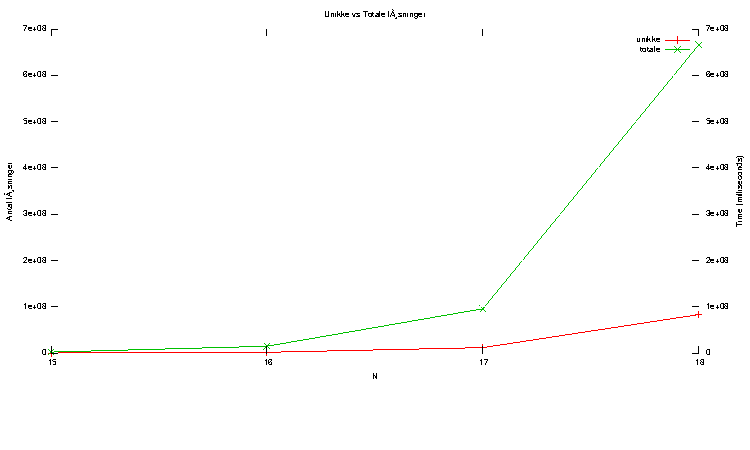
\includegraphics{../benchmarks/unikkevstotale.pdf}
%\caption{Unikke og totale antal løsninger} 
%\label{figur:unikkevstotale}
%\end{center}
%\end{figure}

Som før nævnt er de foregående tests er kørt med java-kode der bruger \texttt{int} til at gemme resultaterne,
i de næste tests er \texttt{int} skiftet ud med \texttt{BigInteger} 

Som det kan ses på figur \ref{figur:lokal} kører den rekursive kode en smule
langsommere med \texttt{BigInteger} end med \texttt{int}, hvor tiden stiger fra
406.065 til 414.238, hvilket svarer til en forøgelse
på knap 2\%. For den iterative udgave af koden stiger tiden fra 700.887 til
736.157, hvilket svarer til en forøgelse på 5\% 

Til sidst har vi kørt java-kode, hvor der bliver brugt \texttt{longs} til
resultaterne. Her er den rekursive udgave en smule hurtigere med \texttt{longs}
i forhold til \texttt{int}. For den iterative udgave er udgaven med
\texttt{longs} en smule langsommere end \texttt{int} 

\subsection{Antal valg}

For at sammenligne om de forskellige udgaver af koden, laver det samme antal
valg, kan man i c-koden og den første 2 udgaver af java-koden \ref{nqueenc},
\ref{nqueensl} og \ref{cornerboard}, tælle antallet af kald til backtrack og
sammenligne dem.  I den iterative udgave er det i stedet antallet af iterationer
i while loopet på linie 90 i \ref{middleboard}. For den rekursive java-kode
tæller vi igen kald til backtrack. Hvis man gør dette med $maxSteps=0$ for vores
kode, kan man se at antallet af iterationer/kald til backtrack er det samme (se
tabel \ref{tabel:backtrackkald}. Som tidligere nævnt kører den iterative kode
væsentligt langsommere end den rekursive. Dette skyldes altså ikke at der bliver
lavet flere iterationer, men derimod at mængden af arbejde der udføres hver
iteration er væsentlig større. Man kunne derfor kigge på hvordan koden i while
loop'et kan optimeres Det skal dog lige nævnes, at med $maxSteps>0$ får vi færre
kald til backtrack/iterationer, hvilket skyldes at en del af disse kald bliver
lavet i forbindelse med oprettelsen af de ekstra boards. 

\begin{table}[h]
\begin{center}
\begin{tabular}{|c|c|c|}
\hline kodebase  & hjørnebræt & midtebræt \\
\hline C kode    &  748267           &  5293206           \\
\hline Java      &  748267           &  5293206           \\
\hline Java rek. &  748267           &  5293206           \\
\hline Java ite. &  748267           &  5293206           \\
\hline
\end{tabular}
\caption{Antal valg for $n=14$}
\label{tabel:backtrackkald}
\end{center}
\end{table}


\subsection{Andel af hjørnebræt vs. midterbræt}
I tabel  \ref{andelHvsM} Andelen af midterbræt ses en oversigt over andelen af midterbræt. Da der bruges mest tid i midterbræt, vil selv små optimeringer og bedre opdelingsstrategi for midterbræt give en bedre global forbedring i forhold til forbedringer for hjørnebræt\footnote{Amdahls lov}. 

\begin{table}[h!]\label{andelHvsM}
\begin{center}
\begin{tabular}{|c|c|}
\hline N & Andel af midterbræt \\
\hline 15 & 89\% \\ 
\hline 16 & 90\% \\
\hline 17 & 91\% \\
\hline 18 & 91\% \\
\hline
\end{tabular}	
\end{center}
\end{table}
 
\subsection{Generering af jobs}

Det skal bemærkes at indsendelse af jobs afhænger af nethastigheden. Tiden for
generering og indsendelse af de forskellige jobs har svinget fra 4ms til 1252ms
(se tabel \ref{tabel:boardgenerering}. Langt den største delaf tiden går også med
at sende jobsne da genereringen af jobs for større mængder jobs tager ca
0.01ms/job

\begin{table}
\begin{center}
\begin{tabular}{|c|c|c|c|c|}
\hline N & maxSteps & tid (ms) & bræt & tid (ms) /bræt \\
\hline 17 & 0 & 4 & 21 & 0.19 \\
\hline 17 & 1 & 6 & 243 & 0.02 \\
\hline 17 & 2 & 23 & 2282 & 0.01 \\
\hline 17 & 3 & 206 & 18161 & 0.01 \\
\hline 17 & 4 & 1252 & 121116 & 0.01 \\
\hline 18 & 0 & 4 & 23 & 0.17 \\
\hline 18 & 1 & 6 & 239 & 0.02 \\
\hline 18 & 2 & 44 & 2983 & 0.01 \\
\hline 18 & 3 & 280 & 26204 & 0.01 \\
\hline
\end{tabular}
\caption{Tid for generering af bræt}
\label{tabel:boardgenering}
\end{center}
\end{table}

\subsection{Kørsel på \mig}

Den tid det tager at løse problemet på \mig\ fra start til slut findes ved at
tage \texttt{Queued} tiden for det første job der er blevet sat i kø, og
\texttt{Finished} tiden for det sidste job der er blevet færdigt, og så finde
forskellen.  På figur \ref{figur:mig} og figur \ref{figur:mig1} kan man se hvor lang beregningstiden er og
hvor lang den reelle tid er for $n=18$ og $maxSteps=0,1$. Ved $maxSteps=0$
ses det at den reelle tid er næsten det dobbelte af beregningstiden. Når
$maxSteps$ bliver sat op til 1 og der dermed bliver genereret flere jobs, kommer
der et noget større overhead, som det kan ses på figuren. På figuren ses det
også at den reelle tid for den iterative udgave er væsentlig højere end for
den rekursive udgave. Dette skyldes at der har været sat 2 forskellige tests
igang på samme tid, og nogle af de jobs fra den pågældende test er blevet
stoppet og sat i kø igen. De er dermed kommet bagest i køen og først blevet kørt
efter den anden test er færdig. Det skal lige nævnes at disse tests alle er kørt
med kun 1 ressource.

\begin{figure}[h]
\begin{center}
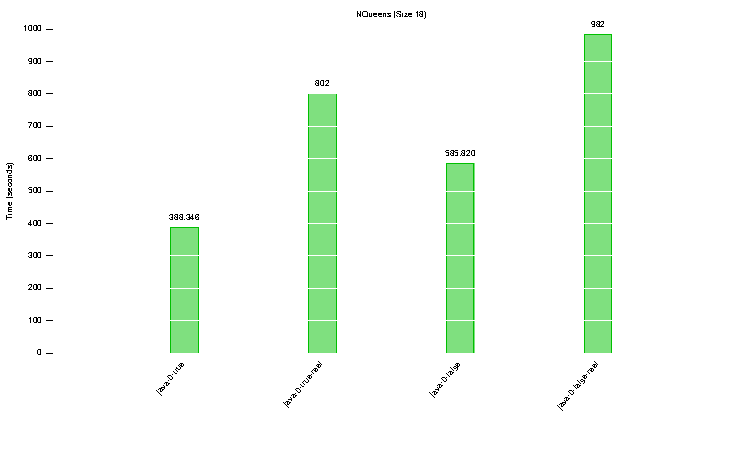
\includegraphics{../benchmarks/mig.pdf}
\caption{NQueen kørt på \mig, for $n=18$ og $maxSteps=0$, true er den
rekursive udgave og false den iterative. Reel står for tiden fra det første job
blev queued til det sidste job er finished}
\label{figur:mig}
\end{center}
\end{figure}

\begin{figure}[h]
\begin{center}
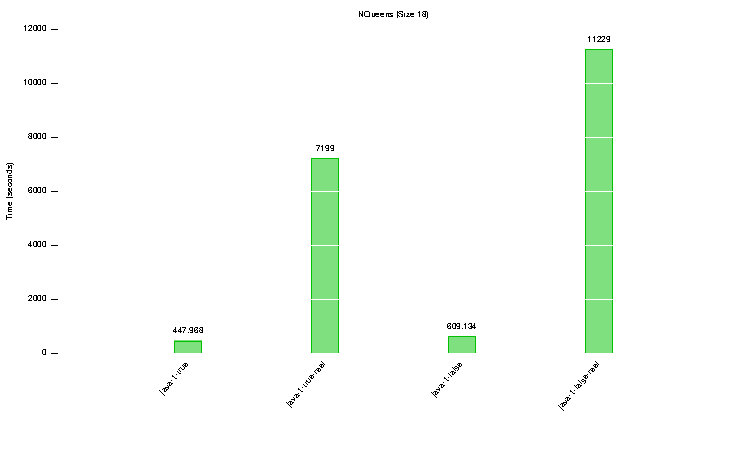
\includegraphics{../benchmarks/mig1.pdf}
\caption{NQueen kørt på \mig, for $n=18$ og $maxSteps=1$, true er den
rekursive udgave og false den iterative. Reel står for tiden fra det første job
blev queued til det sidste job er finished}
\label{figur:mig1}
\end{center}
\end{figure}



\subsubsection{Overhead ved jobskifte}

I MiG\_main() metoden i NQueenJob laver vi et timestamp i starten og slutningen
af metoden.  og kan så tage start tiden for et job og trække sluttiden for det
foregående job fra, og man har så et estimat for hvor lang tid et jobskifte
tager, vi har gjort dette for 8 jobs, og får så 7 estimater, gennemsnittet af
dem bliver 18.455 sek.  Op til 15 af disse 18 sekunder, skyldes at oneclick
applet'en sover i 15 sekunder.  Ved en kørsel med $n=18$ og $maxSteps=1$, hvor
vi så får 289 jobs, giver det knap 89 minutter ved kørsel på én ressource. En del af dette overhead vil
selvfølgelig blive "gemt", når der er flere ressourcer der kører samtidigt.

